
\glssetexpandfield{desc} %Comando para expandir otros comandos en la descripcion de los glosarios
\glssetexpandfield{name} %Comando para expandir otros comandos en el nombre de los glosarios
%==========================CONTADORES==============================%
%Se crea nuevo contador que se utiliza para agregar las letras correspondientes a los anexos
\newcounter{anexosletra}

%Se establece 1 como el valor inicial del contador
\setcounter{anexosletra}{1}

%Se crea el contador que se utiliza para agregar el numero correlativo de las secciones dentro de un anexo
\newcounter{anexosseccion}

%Se crea el contador que se utiliza para agregar el numero correlativo de una subseccion dentro de un anexo
\newcounter{anexossubseccion}

%Se crea el contador que se utiliza para llevar la cuenta de cuantos autores han sido ingresados en la primera portada, esto sirve para saber si la mayoria son hombres o mujeres y tambien para establecer un maximo de cuatro autores
\newcounter{contadorautor}

%Se establece el valor inicial 0 para el contador de autores
\setcounter{contadorautor}{0}

%Se crea el contador que se utiliza para llevar la cuenta de cuantos autores son hombres
\newcounter{contadorhombres}

%Se establece el valor inicial 0 para el contador de hombres
\setcounter{contadorhombres}{0}

%Se crea el contador que se utiliza para llevar la cuenta de cuantos autores son mujeres
\newcounter{contadormujeres}

%Se establece el valor inicial 0 para el contador de mujeres
\setcounter{contadormujeres}{0}

%
\newcounter{resultadosexosautores}
\setcounter{resultadosexosautores}{0}

\newcounter{figuras}
\setcounter{figuras}{0}

%===========================COMANDOS=============================%

%Este comando verifica que el parametro que le pasaron este vacio o no
\newcommand{\verificarvacio}[3]{
    \ifdefined #1
        \ifthenelse{\equal{#1}{}}{%
        %Si esta vacio muestra un mensaje de advertencia en mayuscula y de color rojo
        \textcolor{red}{\MakeUppercase{#2}}%
        }{
        %Si no esta vacio entonces muestra el texto del parametro en mayuscula
        \MakeUppercase{#1}
        }
    \else
        \textcolor{red}{\MakeUppercase{#3}}
    \fi
}

% Estos comandos guardan los nombres de los integrantes del grupo, el comando autorA corresponde al primer autor, autorB corresponse al segundo autor, autorC corresponde al tercer autor y autorD corresponde al cuarto autor
\newcommand{\autorA}{}
\newcommand{\autorB}{}
\newcommand{\autorC}{}
\newcommand{\autorD}{}

%El comando autor se encarga de agregar los nombres de los autores en los comandos anteriores
\newcommand{\autor}[2]{
    %Se verifica cuantas veces se a utilizado el comando autor, si se ha hecho menos de cuatro veces entonces todavia se pueden agregar mas autores, si se ha hecho igual o mas de cuatro veces entonces ya no se puede agregar mas autores
    \ifthenelse{\value{contadorautor} < 4}{
        %El contador "contadorautor" sirve para llevar la cuenta de cuantos autores se han ingresado, el comando \ifcase sirve para verificar que valor tiene el contador en ese momento y en base a eso hacer una acción u otra.
        \ifcase\value{contadorautor}%
            %Si el contador es 0 no se ha ingresado ningun autor todavia, por lo tanto se agrega el nombre al comando autorA
            \renewcommand{\autorA}{#1}
        \or%
            %Si el contador es 1 se ha ingresado ya un autor, por lo tanto se agrega el nombre al comando autorB
            \renewcommand{\autorB}{#1}
        \or%
            %Si el contador es 2 se han ingresado dos autores, por lo tanto se agrega el nombre al comando autorC
            \renewcommand{\autorC}{#1}
        \or%
            %Si el contador es 3 se han ingresado tres autores, por lo tanto se agrega el nombre al comando autorD
            \renewcommand{\autorD}{#1}
        \fi

        %Se valida que el sexo ingresado para cada un autor sea hombre o mujer, si es mujer el contador "contadormujeres" incrementa en 1, si en hombre el contador "contadorhombres incrementa en 1
        \ifthenelse{\equal{#2}{M}}{
            \stepcounter{contadormujeres}
        }{
            \stepcounter{contadorhombres}
        }

        %Se incrementa en 1 el contador "contadorautor" al final del comando
        \stepcounter{contadorautor}
    }{
    
    }
}

%Este comando sirve para verificar el numero de mujeres y hombres en el grupo de trabajo ya que es necesario para escribir el grado a optar en la primera portada del trabajo
\newcommand{\verificarsexoautores}{
    \ifthenelse{\equal{\value{contadormujeres}}{0}}{
        %Si no hay mujeres en el grupo entonces el valor del contador resultadosexosautores es 1
        \setcounter{resultadosexosautores}{1}
    }{
        \ifthenelse{\equal{\value{contadorhombres}}{0}}{
            %Si no hay hombres en el grupo entonces el valor del contador resultadosexosautores es 2
            \setcounter{resultadosexosautores}{2}
        }{
            \ifthenelse{\value{contadorhombres} > \value{contadormujeres} }{
                %Si hay mas hombres que mujeres entonces el valor de resultadosexosautores es 3
                \setcounter{resultadosexosautores}{3}
            }{
                \ifthenelse{\value{contadormujeres} > \value{contadorhombres}}{
                    %Si hay mas mujeres que hombres entonces el valor de resultadosexosautores es 4
                    \setcounter{resultadosexosautores}{4}
                }{
                    \ifthenelse{\equal{\value{contadorhombres}}{\value{contadormujeres}}}{
                        %Si hay igual numero de mujeres que de hombres el valor del contadore resultadosexosautores es 5
                        \setcounter{resultadosexosautores}{5}
                    }{
                    
                    }
                }
            }
        }
    }
}

%Valor booleano para saber si ya se ingreso alguna entrada a las siglas o no
\newcommand{\ningunasiglaingresada}{true} 

%Este comando sirve para agregar nuevas siglas a la seccion de siglas
\newcommand{\itemsiglas}[2]{%
    %Valida que se agreguen entradas a las siglas solo si los dos parametros del comando \itemsiglas han sido llenados, si no han sido llenados no se agreaga ninguna sigla nueva
    \ifthenelse{\equal{#1}{} \or \equal{#2}{}}{ 
    
    }{
    %Si los dos parametros fueron agregados entonces se ingresa la nueva sigla y \ningunasiglaingresada cambia a falso
        \renewcommand{\ningunasiglaingresada}{false}
        \newglossaryentry{#1}{name={#1}, type=siglas, description={#2}}%
    }
}

%Valor booleano para saber si ya se ingreso alguna entrada a las abreviaturas o no
\newcommand{\ningunaabreviaturaingresada}{true} 

%Este comando sirve para agregar nuevas abreviaturas a la sección de abreviaturas
\newcommand{\itemabreviatura}[2]{
    %Valida que se agreguen entradas a las abreviaturas solo silos dos parametros del comando \itemabreviatura han sido llenados, si no han sido llenados no se agreaga ninguna abreviatura nueva
    \ifthenelse{\equal{#1}{} \or \equal{#2}{}}{  
    }{
    %Si los dos parametros fueron agregados entonces se ingresa la nueva abreviatura y \ningunaabreviaturaingresada cambia a falso
        \renewcommand{\ningunaabreviaturaingresada}{false}
        \newglossaryentry{#1}{name={#1}, type=abreviaturas, description={#2}}%
    }
    
}

%Valor booleano para saber si ya se ingreso alguna entrada a la nomenclatura o no
\newcommand{\ningunanomenclaturaingresada}{true}

%Este comando sirve para agregar un nuevo elemento a la sección de nomenclatura
\newcommand{\itemnomenclatura}[2]{%
    %Valida que se agreguen entradas a la nomenclatura solo silos dos parametros del comando \itemnomenclatura han sido llenados, si no han sido llenados no se agreaga ninguna nomenclatura nueva
    \ifthenelse{\equal{#1}{} \or \equal{#2}{}}{       
    }{
    %Si los dos parametros fueron agregados entonces se ingresa la nueva nomenclatura y \ningunanomenclaturaingresada cambia a falso
        \renewcommand{\ningunanomenclaturaingresada}{false}
        \newglossaryentry{#2}{name={#1}, type=nomenclatura, description={#2}}%
    }
}

%Valor booleano para saber si ya se ingreso alguna entrada al glosario o no
\newcommand{\glosariovacio}{true} 

%Este comando sirve para agregar nuevas palabras al glosario
\newcommand{\itemglosario}[2]{%
    %Valida que se agreguen entradas al glosario solo si los dos parametros del comando \glosario han sido llenados, si no han sido llenados no se agreaga ninguna entrada al glosario nueva
    \ifthenelse{\equal{#1}{} \or \equal{#2}{}}{ 
        
    }{
    %Si los dos parametros fueron agregados entonces se ingresa la nueva
    %entrada del glosario y \glosariovacio cambia a falso
        \renewcommand{\glosariovacio}{false}
        \newglossaryentry{#1}{name={#1}, type=glosario, description={#2}}%
    }
}


%Este comando esta creado para hacer uno o dos saltos de pagina dependiendo de si la seccion termina en pagina impar o par
\newcommand{\paroimpar}[1]{
    \pgfmathparse{mod(#1,2)}
    \edef\resultado{\pgfmathresult}% Almacenar el resultado como una macro expandida

    \ifthenelse{\equal{\resultado}{0.0}}{
        \newpage
    }{
        \newpage
        \null\thispagestyle{empty}
        \newpage
    }
}

%Comando utilizado para crear los capitulos
\newcommand{\capitulo}[2]{
    \begin{capituloentorno}
    {
        #1
    }{
        #2
    }
    \end{capituloentorno}
}

%Valor booleano para saber si ya se agrego una imagen al documento o no
\newcommand{\ningunaimageningresada}{true}

% Se crea nuevo comando que establece el formato de las figuras
\newcommand{\imagen}[6]{
    \renewcommand{\ningunaimageningresada}{false}
    %Se valida si existe alguna imagen con el nombre proporcionado
    \IfFileExists{img/#1}{
        %Se cambia el valor del comando ningunaimageningresada a false
        \renewcommand{\ningunaimageningresada}{false}
        %\stepcounter{figuras}
        %Si el cuarto parametro del comando es V significa que se quiere mostrar la imagen en formato vertical.
        \ifthenelse{\equal{#6}{V}}{
            %Se valida que el tercer parametro no este vacio, el tercer parametro corresponde a la escala que tendra la figura, si el parametro esta vacío entonces se coloca 1 por defecto
            \ifthenelse{\equal{#5}{}}{
                \begin{figure}[H]
                \vspace{2\baselineskip}
                \centering
                \includegraphics[scale=1]{img/#1}
                \ifthenelse{\equal{#3}{true}}{
                    \caption[#2]{#2. Adaptado de: [#4]}
                }{
                    \caption[#2]{#2. Fuente: [#4]}
                }
                \label{fig:#1}
                \end{figure}
            }{
            %Si no esta vacio entonces se coloca el valor que se escribio en el tercer parametro
                \begin{figure}[H]
                \vspace{2\baselineskip}
                \centering
                \includegraphics[scale=#5]{img/#1}
                \ifthenelse{\equal{#3}{true}}{
                    \caption[#2]{#2. Adaptado de: [#4]}
                }{
                    \caption[#2]{#2. Fuente: [#4]}
                }
                \label{fig:#1}
                \end{figure}
            }    
        }{
        %Si el cuarto parametro es H significa que la figura se mostrara de manera horizontal
        \ifthenelse{\equal{#6}{H}}{
            \begin{sidewaysfigure}
                \includegraphics[width=\linewidth]{img/#1}
                \ifthenelse{\equal{#3}{true}}{
                    \caption[#2]{#2. Adaptado de: [#4]}
                }{
                    \caption[#2]{#2. Fuente: [#4]}
                }
                \label{fig:#1}
            \end{sidewaysfigure}
        }{
        \textcolor{red}{\MakeUppercase{ERROR: el parametro para la orientacion de la imagen solo puede ser 'H' para horizontal y 'V' para vertical}}
        }
        }
    }{
        \textcolor{red}{\MakeUppercase{ERROR: la imagen con nombre #1 no existe}}
    }
}

%Este comando sirve para escribir la carrera que se esta cursando de la manera correcta en la primera porta validando la cantidad de mujeres y hombres en el grupo
\newcommand{\determinarcarrera}[2]{
    %Si el segundo parametro del comando es 1 significa que se inserata el nombre de la carrera en la segunda portada en la parte del director de carera
    \ifthenelse{\equal{#2}{1}}{%
        %El primer parametro indica la carrera que se esta cursando
        \ifcase #1%
            INGENIERÍA INFORMÁTICA%
        \or%
            INGENIERÍA CIVIL%
        \or%
            INGENIERÍA ELÉCTRICA%
        \or%
            INGENIERÍA ENERGÉTICA%
        \or%
            INGENIERÍA DE ALIMENTOS%
        \or%
            INGENIERÍA QUÍMICA%
        \or%
            INGENIERÍA MECÁNICA%
        \or%
            INGENIERÍA INDUSTRIAL%
        \or%
            ARQUITECTURA%
        \or%
            LICENCIATURA EN DISEÑO%
        \else%
            \textcolor{red}{ERROR: NO SE HA INGRESADO UN NUMERO VALIDO PARA LA CARRERA}%
        \fi%
    }{%
    %Si el segundo parametro no es 1 significa que se esta insertando el nombre de la carrera en la parte donde se menciona el grado que se quiere obtener en la primera portada

    %Si el valor del contador resultadosexosautores es 1 entonces solamente hay hombres en el grupo y se pone de la siguiente manera
    \ifthenelse{\equal{\value{resultadosexosautores}}{1}}{
        \ifcase #1%
            INGENIERO INFORMÁTICO\\%
        \or%
            INGENIERO CIVIL\\%
        \or%
            INGENIERO ELECTRICISTA\\%
        \or%
            INGENIERO ENERGÉTICO\\%
        \or%
            INGENIERO DE ALIMENTOS\\%
        \or%
            INGENIERO QUÍMICO\\%
        \or%
            INGENIERO MECÁNICO\\%
        \or%
            INGENIERO INDUSTRIAL\\%
        \or%
            ARQUITECTO\\%
        \or%
            LICENCIADO EN DISEÑO\\%
        \else%
            \textcolor{red}{ERROR: NO SE HA INGRESADO UN NUMERO VALIDO PARA LA CARRERA}%
        \fi%
    }{
            %Si el valor del contador "resultadosexosautores" es 2 entonces solamente hay mujeres en el grupo y se pone de la siguiente manera
            \ifthenelse{\equal{\value{resultadosexosautores}}{2}}{
            \ifcase #1%
                INGENIERA INFORMÁTICA\\%
            \or%
                INGENIERA CIVIL\\%
            \or%
                INGENIERA ELECTRICISTA\\%
            \or%
                INGENIERA ENERGÉTICA\\%
            \or%
                INGENIERA DE ALIMENTOS\\%
            \or%
                INGENIERA QUÍMICA\\%
            \or%
                INGENIERA MECÁNICA\\%
            \or%
                INGENIERA INDUSTRIAL\\%
            \or%
                ARQUITECTA\\%
            \or%
                LICENCIADA EN DISEÑO\\%
            \else%
                \textcolor{red}{ERROR: NO SE HA INGRESADO UN NUMERO VALIDO PARA LA CARRERA}%
            \fi%
        }{
            %Si hay mas mujeres que hombres en el grupo entonces el valor del contador "resultadosexosautores" es 3 y se escribe de la siguiente manera 
            \ifthenelse{\equal{\value{resultadosexosautores}}{3} \or \equal{\value{resultadosexosautores}}{5}}{
                \ifcase #1%
                    INGENIERO(A) INFORMÁTICO(A)\\%
                \or%
                    INGENIERO(A) CIVIL\\%
                \or%
                    INGENIERO(A) ELECTRICISTA\\%
                \or%
                    INGENIERO(A) ENERGÉTICO(A)\\%
                \or%
                    INGENIERO(A) DE ALIMENTOS\\%
                \or%
                    INGENIERO(A) QUÍMICO(A)\\%
                \or%
                    INGENIERO(A) MECÁNICO(A)\\%
                \or%
                    INGENIERO(A) INDUSTRIAL\\%
                \or%
                    ARQUITECTO(A)\\%
                \or%
                    LICENCIADO(A) EN DISEÑO\\%
                \else%
                    \textcolor{red}{ERROR: NO SE HA INGRESADO UN NUMERO VALIDO PARA LA CARRERA}%
                \fi%
            }{
                %Si hay mas mujeres que hombres entonces el valor del contador "resultadosexosautores" es 4 y se escribe de la siguiente forma
                \ifthenelse{\equal{\value{resultadosexosautores}}{4}}{%
                \ifcase #1%
                    INGENIERA(O) INFORMÁTICA(O)\\%
                \or%
                    INGENIERA(O) CIVIL\\%
                \or%
                    INGENIERA(O) ELECTRICISTA\\%
                \or%
                    INGENIERA(O) ENERGÉTICA(O)\\%
                \or%
                    INGENIERA(O) DE ALIMENTOS\\%
                \or%
                    INGENIERA(O) QUÍMICA(O)\\%
                \or%
                    INGENIERA(O) MECÁNICA(O)\\%
                \or%
                    INGENIERA(O) INDUSTRIAL\\%
                \or%
                    ARQUITECTA(O)\\%
                \or%
                    LICENCIADA(O) EN DISEÑO\\%
                \else%
                    \textcolor{red}{ERROR: NO SE HA INGRESADO UN NUMERO VALIDO PARA LA CARRERA}%
                \fi%
            }{}
            }
        }
    } 
    }
}

%Valor booleano para validar si ninguna tabla ha sido ingresada
\newcommand{\ningunatablaingresada}{true}

%Este comando sirve para insertar una tabla en el documento utlizando el formato requerido
\newcommand{\tabla}[2]{
    %El valor del comando "ningunatablaingresada" cambia a false y que se esta ingresando una tabla
    \renewcommand{\ningunatablaingresada}{false}
    %Se valida si la tabla se esta ingresando de forma vertical u horizontal
    \ifthenelse{\equal{#1}{V}}{
        #2
    }{
    \ifthenelse{\equal{#1}{H}}{
        \begin{landscape}
            #2
        \end{landscape}
    }{
    \textcolor{red}{\MakeUppercase{ERROR: el parametro para la orientacion de la tabla solo puede ser 'H' para horizontal y 'V' para vertical}}
    }
    }
}

%Este comando se encarga de crear la portada de un anexo
\newcommand{\portadanexo}[1]{
    \thispagestyle{empty}
    \vspace*{\fill}
    {\centering{\fontsize{20}{0}\selectfont ANEXO \, \MakeUppercase{\alph{anexosletra}\\}}
    {\fontsize{16}{24}\selectfont \MakeUppercase{#1}\\}}
    \vspace*{\fill}
    \newpage
    \null
    \thispagestyle{empty}
    \newpage
}

%Este comando crea el cuerpo de un anexo
\newenvironment{cuerpoanexo}[1]{
    \setlength{\parskip}{\baselineskip}
    \setcounter{page}{1}
    \renewcommand{\thepage}{\MakeUppercase{\alph{anexosletra}}-\arabic{page}}
    #1
    \newpage
}{
   
}

%Este comando sirve para crear un anexo
\newcommand{\anexo}[2]{
    \chapter*{\phantom{Anexo \theanexosletra}}
    \setcounter{numeroimagenesanexos}{1}
    \setcounter{anexosseccion}{0}
    
    \addtocontents{toc}{%
      ANEXO \MakeUppercase{\alph{anexosletra}}.\hspace{1em}%
      \parbox[t]{380pt}{\strut#1\strut}\\
    }
    \portadanexo{#1}
    \begin{cuerpoanexo}{
        #2
    }
    
    \end{cuerpoanexo}
    \stepcounter{anexosletra}

}

%Este comando sirve para agregar imagenes en los anexos utilizando el formato adecuado
\newcommand{\imagenanexo}[4]{
    \IfFileExists{img/#1}{
        \ifthenelse{\equal{#4}{V}}{
            \ifthenelse{\equal{#3}{}}{
                \begin{figure}[H]
                \vspace{2\baselineskip}
                \centering
                \includegraphics[scale=1]{img/#1}
                \caption*{Figura \Alph{anexosletra}.\arabic{numeroimagenesanexos} #2}
                \label{fig:#1}
                \end{figure}
            }{
                \begin{figure}[H]
                \vspace{2\baselineskip}
                \centering
                \includegraphics[scale=#3]{img/#1}
                \caption*{Figura \Alph{anexosletra}.\arabic{numeroimagenesanexos} #2}
                \label{fig:#1}
                \end{figure}
            }    
        }{
        \ifthenelse{\equal{#4}{H}}{
            \begin{sidewaysfigure}
                \centering
                \includegraphics[width=\linewidth]{img/#1}
                \caption*{Figura \Alph{anexosletra}.\arabic{numeroimagenesanexos} #2}
                \label{fig:#1}
            \end{sidewaysfigure}
        }{
        \textcolor{red}{\MakeUppercase{ERROR: el parametro para la orientacion de la imagen solo puede ser 'H' para horizontal y 'V' para vertical}}
        }
        }
        \stepcounter{numeroimagenesanexos}
    }{
        \textcolor{red}{\MakeUppercase{ERROR: la imagen con nombre #1 no existe}}
    }
}

%Este comando sirve para hacer referencia a una figura utilizando el formato correcto
\newcommand{\reffig}[1]{
    Figura \ref{fig:#1}%
}

%Este comando sirve para hace referencia a una tabla utilizando el formato correcto
\newcommand{\reftab}[1]{
    Tabla \ref{#1}%
}

%Este comando permite agregar secciones en los anexos con el formato correcto
\newcommand{\sectionanexo}[1]{
    \stepcounter{anexosseccion}%\\
    \textbf{\Alph{anexosletra}.\theanexosseccion \, #1}%\\
    %\\
    \setcounter{anexossubseccion}{0}
}

%Este comando sirve para escribir una subseccion en los aexos utilizando el formato adecuado
\newcommand{\subsectionanexo}[1]{
    \stepcounter{anexossubseccion}
    \textbf{\Alph{anexosletra}.\theanexosseccion.\theanexossubseccion \, #1}%\\
    %\\
}

%Este comando sirve para escribir la fuente de las tablas de manera apropiada
\newcommand{\fuentetabla}[1]{
    \caption*{Fuente: [#1]}
}

%Este comando sirve para escribir el epigrafe de una tabla que continua en la pagina siguiente y por lo tanto se debe colocar la palabra continución
\newcommand{\captioncontinuacion}[1]{
    \caption*{Tabla \thetable \, #1 (continuación)}
}



% --- PAQUETES ADICIONALES ---
\usepackage{pgfgantt}
\usepackage{pgfplots}
\pgfplotsset{compat=1.18}

\definecolor{myorange}{RGB}{255, 170, 50}
\definecolor{mylightorange}{RGB}{255, 190, 90}
\definecolor{myblue}{RGB}{65, 105, 225}
\definecolor{mygreen}{RGB}{180, 230, 130}
\definecolor{titleblue}{RGB}{60, 90, 200}
\definecolor{headergreen}{RGB}{195, 230, 140}

% ================================================================
%            Sección editable para primera portada
% ================================================================
% =============== NO MODIFICAR LOS COMANDOS ======================
% ================================================================

\newcommand{\titulo}{IMPLEMENTACIÓN DE PROTOTIPO PARA ``UCACHAT''} %Título del trabajo

% 0. Informatica
% 1. Civil
% 2. Electrica
% 3. Energetica
% 4. Alimentos
% 5. Quimica
% 6. Mecanico
% 7. Industrial
% 8. Arquitectura
% 9. Licenciatura en Diseño
\newcommand{\carrera}{0}

\autor{WALTER RAFAEL MORALES HENRIQUEZ}{H} % Autor 1
\autor{MONICA ALEJANDRA VEGA FLORES}{M} % Autor 2 (opcional)
\autor{OMAR ALFREDO VASQUEZ ESCAMILLA}{H} % Autor 3 (opcional)
\autor{RENE ARMANDO FLORES CORTEZ}{H} % Autor 4 (opcional)


\newcommand{\mesdegraduacion}{Mes y año de graduación} % Mes y año de graduación

%================================================================
%            Sección editable para segunda portada
% ===============================================================
% ================ NO MODIFICAR LOS COMANDOS ====================
% ===============================================================

\newcommand{\rector}{Nombre del rector}% Nombre del rector
\newcommand{\sexorector}{masculino} % Sexo del secretario o secretaria general
\newcommand{\secretariogeneral}{Nombre del secretario o secretaria general} % Nombre del secretario o secretaria general
\newcommand{\sexosecretario}{masculino} % Sexo del secretario o secretaria general
\newcommand{\decano}{Nombre del decano de la facultad de ingeniería y arquitectura} % Nombre del decano de la facultad de ingeniería y arquitectura
\newcommand{\sexodecano}{masculino} % Sexo del secretario o secretaria general
\newcommand{\directordecarrera}{Nombre del director de la carrera} % Director de la carrera
\newcommand{\sexodirectordecarrera}{masculino} % Sexo del secretario o secretaria general
\newcommand{\directordetrabajo}{Nombre del director del trabajo de graduación} % Director del trabajo de graduación
\newcommand{\sexodirectordetrabajo}{masculino} % Sexo del secretario o secretaria general
\newcommand{\lector}{Nombre del lector o lectora} % Nombre del lector o lectora
\newcommand{\sexolector}{masculino} % Sexo del lector o lectora

%=================================================================
%            Sección editable para agradecimientos
% ================================================================
% ================ NO MODIFICAR LOS COMANDOS =====================
% ================================================================
\newcommand{\agradecimiento}{}
%\newcommand{\agradecimiento}{En esta sección el grupo puede agradecer a las personas que ayudaron en el proceso de creación de la tesis. Esta seccion es opcional y es realizada por todo el grupo, y su extensión no debe ser mayor a una página.} % Agradecimientos

%=================================================================
%               Sección editable para dedicatorias
% ================================================================
% ================= NO MODIFICAR LOS COMANDOS ====================
% ================================================================
\newcommand{\dedicatoriaautorA}{}
%\newcommand{\dedicatoriaautorA}{En esta sección los estudiantes pueden dedicar a sus familiares o seres querido el esfuerzo realizado durante la realización del trabajo y en general durante toda la carrera, así como también agradecer a las personas que los han apoyado durante este proceso. Las dedicatorias son opcionales, cada estudiante decide la escribe o no y la extensión de la dedicatoria no debe ser mayor a una página.}% Dedicatoria del autor A, ingresar solo si se ingreso "true" en el comando "porcadaestudiante".

\newcommand{\dedicatoriaautorB}{}% Dedicatoria del autor B, ingresar solo si se ingreso "false" en el comando "porcadaestudiante".

\newcommand{\dedicatoriaautorC}{}% Dedicatoria del autor C, ingresar solo si se ingreso "false" en el comando "porcadaestudiante".

\newcommand{\dedicatoriaautorD}{}% Dedicatoria del autor D, ingresar solo si se ingreso "false" en el comando "porcadaestudiante".

%=================================================================
%                   Sección editable para resumen
% ================================================================
% ================== NO MODIFICAR LOS COMANDOS ===================
% ================================================================

\newcommand{\resumen}{La comunidad estudiantil de la Universidad Centroamericana José Simeón Cañas (UCA) enfrenta el desafío de acceder a información institucional, la cual se encuentra dispersa en múltiples fuentes y formatos. Esta descentralización genera ineficiencias, pérdida de tiempo y desinformación al realizar consultas sobre procesos académicos, administrativos y servicios universitarios. El presente proyecto aborda esta problemática mediante la implementación de un prototipo de asistente conversacional denominado ``UCAchat''.

La solución se basa en una arquitectura de Retrieval-Augmented Generation (RAG), que potencia un Large Language Model (LLM) con una base de conocimiento específica, construida a partir de documentos públicos de la universidad. La metodología propuesta comprende tres fases: una investigación inicial para recopilar documentos y determinar las necesidades de los estudiantes a través de encuestas; el diseño y desarrollo del prototipo RAG y su interfaz web; y una fase final de pruebas y evaluación con usuarios para medir su eficacia y pertinencia. Se espera que el prototipo demuestre la viabilidad de centralizar la información institucional y mejorar significativamente la experiencia estudiantil.
}

%=================================================================
%                  Sección editable para siglas
% ================================================================
% ================== NO MODIFICAR LOS COMANDOS ===================
% ================================================================

\itemsiglas{Siglas}{En esta sección se deben escribir las siglas que se utilizan en el trabajo. Una sigla es una palabra conformada por las iniciales de un nombre o expresión compuesta por varias palabras, por ejemplo ONU (Organización de las Naciones Unidas).}

%=================================================================
%                 Sección editable para abreviaturas
% ================================================================
% ================== NO MODIFICAR LOS COMANDOS ===================
% ================================================================

\itemabreviatura{Abreviaturas}{En esta sección se deben escribir las abreviaturas que se utilizan en el trabajo. Las\newline abreviaturas son representaciones reducidas de una palabra, por ejemplo\newline Sr.(Señor), no se debe abusar de ellas y no se deben colocar las unidades de medida.}
\itemabreviatura{}{}
\itemabreviatura{}{}

%=================================================================
%               Sección editable para nomenclatura
% ================================================================
% ================== NO MODIFICAR LOS COMANDOS ===================
% ================================================================

\itemnomenclatura{Nomenclaturas}{En esta sección se debe escribir la nomenclatura que se utiliza en el trabajo. La nomenclatura son los diferentes símbolos que se utilizan en un ámbito especifico de las ciencias, por ejemplo en el área de química $H2O$(formula del agua) o en física $V$(Voltaje).}
\itemnomenclatura{}{}
\itemnomenclatura{}{}

%=================================================================
%          Sección editable para capítulo de introcuccion
% ================================================================
% ================== NO MODIFICAR LOS COMANDOS ==================
% ===============================================================

\newenvironment{planteamientodelproblema}{
Los estudiantes de la Universidad Centroamericana José Simeón Cañas, y las personas interesadas en estudiar en esta universidad, deben realizar a lo largo de su carrera diferentes procesos, tanto administrativos como educativos, sociales y recreativos. La cantidad de información existente impide su centralización, por lo cual muchos estudiantes desconocen los lineamientos que deben seguir, los lugares a los que deben acercarse y, en general, dónde encontrar la información que necesitan.

Esto provoca que los estudiantes enfrenten dificultades para acceder de manera rápida y eficiente a datos relevantes como horarios de la cafetería, reglamentos institucionales, mallas curriculares, servicios disponibles dentro de la institución, así como opciones de alimentación cercanas al campus. La falta de un sistema centralizado de consulta genera pérdida de tiempo, desinformación y, en algunos casos, desmotivación en la comunidad universitaria.

Ante esta situación, surge la necesidad de contar con una herramienta digital que concentre y organice la información más relevante en un solo lugar, de manera accesible, práctica y actualizada.
}{}
\newenvironment{antecedentes}{
\textbf{Chatbot para la educación: un asistente conversacional sobre inteligencia artificial.} \\
Los autores Gil, F., Moraes, A. y Tift, W. de la Universidad de la República (Uruguay) en su trabajo de graduación para optar por el título de Ingeniero en Computación.

Colibri, un chatbot educativo de código abierto diseñado para apoyar a docentes en la enseñanza y comprensión de la inteligencia artificial generativa. El sistema se entrenó con fuentes confiables, integrando funcionalidades que permiten responder preguntas, 
brindar ejemplos y recomendar lecturas sobre IA. Además, buscó fomentar un aprendizaje autónomo mediante una interfaz conversacional intuitiva. Este antecedente resulta relevante porque muestra cómo los chatbots pueden ser empleados en el ámbito educativo para transmitir conocimiento especializado de manera clara y accesible \cite{gil2025chaboteducation}. \\[1em]

\textbf{Chatbot en ámbitos académicos.} \cite{geekoders2019} \\
Los autores Geekoders de la Universidad de El Salvador, sede en Santa Tecla, en su proyecto de graduación para optar por el título de Ingeniero en Software.

Un asistente virtual conversacional accesible a través de Facebook Messenger. El chatbot fue programado con 38 intenciones específicas para atender consultas frecuentes de 
los estudiantes, como inscripciones, horarios, constancias y procesos administrativos. Durante su primera semana de uso, mostró resultados positivos en la cantidad de interacciones realizadas por los alumnos. Este antecedente es importante porque ejemplifica la 
aplicación práctica de chatbots en contextos universitarios para mejorar la comunicación institucional y dar respuestas rápidas a dudas comunes \cite{geekoders2019} . \\[1em]

\textbf{Chatbot for communicating with university students in emergency situations.} \\
Los autores Balderas, A., García-Mena, R. F., Huerta, M., Mora, N., \& Dodero, J. M. de la Universidad de Cádiz en su trabajo de graduación por optar por el título de Ingeniero en Informática.

Un chatbot desarrollado para atender a estudiantes universitarios durante situaciones de emergencia, como la pandemia de COVID-19. El sistema fue diseñado con Dialogflow y entrenado para manejar preguntas frecuentes relacionadas con servicios de apoyo psicológico, 
trámites académicos y acceso a recursos institucionales. Fue evaluado con estudiantes, docentes y personal administrativo, obteniendo resultados positivos en facilidad de uso, rapidez y claridad en las respuestas \cite{balderas2023emergencysituation}.
}{}

\newenvironment{alcances}{
\begin{itemize}
    \item La aplicación será accesible a través de una página web, permitiendo a los estudiantes y demás usuarios consultar información y resolver dudas relacionadas con la universidad de manera centralizada y práctica.
    \item Contará con una interfaz de usuario intuitiva, simple y accesible, diseñada para facilitar la navegación y garantizar que los usuarios, independientemente de su nivel de experiencia tecnológica, puedan interactuar con el sistema sin dificultad.
    \item La aplicación ofrecerá respuestas rápidas y contextualizadas, reduciendo la necesidad de que los estudiantes acudan a múltiples fuentes de información dispersas.
    \item Se incluirá un diseño adaptativo (responsive), que permitirá el acceso tanto desde computadoras de escritorio como desde dispositivos móviles.
\end{itemize}
}{}

\newenvironment{limitaciones}{
La aplicación estará limitada a contestar preguntas relacionadas al contexto de la universidad y sus extensiones, se evitará en la medida de lo posible dar seguimiento a información que esté fuera de estos límites.
}{}
\newenvironment{objetivogeneral}{Implementar un chat con integración de inteligencia artificial para proveer información de manera centralizada acerca de la Universidad Centroamericana José Simeón Cañas y sus procesos.}{}
\newenvironment{objetivosespecificos}{
\begin{itemize}
    \item Identificar los procesos más comunes por los cuales los estudiantes realizan consultas de información, con el fin de recopilar y clasificar sus necesidades principales.
    \item Elaborar una base de conocimiento estructurada que contenga la información académica y administrativa más consultada por los estudiantes.
    \item Analizar diferentes alternativas de modelos de inteligencia artificial que permitan un equilibrio entre eficiencia y uso de recursos.
    \item Integrar la base de conocimiento con un modelo de inteligencia artificial que responda de manera clara y precisa a las consultas estudiantiles.
\end{itemize}

}{}

%=================================================================
%                Sección editable para capítulos
% ================================================================
% ================= NO MODIFICAR LOS COMANDOS ====================
% ================================================================

\newcommand{\capitulos}{
    \capitulo{Estuctura de los capítulos}{
    Los capítulos del Trabajo de Graduación con el tema de Implementación de prototipo para UCAchat están estructurados de la siguiente manera:

    \begin{listaenumerada}
        \item Marco teórico
        \item Metodología
        \item Presentación, análisis e interpretación de resultados
    \end{listaenumerada}
    }
    \capitulo{Marco teórico}{


\section{Orígenes de la Inteligencia Artificial (IA)}

La inteligencia artificial (IA) es una tecnología que ha experimentado un avance espectacular en poco tiempo, gracias a la combinación de factores como el \textit{big data}, el \textit{blockchain}, la nube, el internet de las cosas, la robótica y la realidad virtual. Aunque la IA no es una invención reciente, ya que sus orígenes se remontan a hace más de 50 años, su impacto actual es enorme y afecta a casi todos los ámbitos de la vida. Una conjunción de factores, como los avances en la potencia informática, la disponibilidad de enormes cantidades de datos y nuevos algoritmos, ha permitido que se produzcan grandes logros en los sistemas de IA en los últimos años.

No hay una definición clara de estos sistemas que goce de amplio consenso, porque, de una parte, la IA está sometida a las variaciones que se produzcan como consecuencia de los avances tecnológicos, de forma que no responde a algo estático, sino que es producto de una tecnología disruptiva que, además, se desarrolla a pasos acelerados. De otra parte, no existe un consenso entre los agentes implicados sobre lo que son los sistemas de IA. Sin embargo, con el objeto de regular la inteligencia artificial (IA) de manera efectiva, es necesaria una comprensión común de lo que se entiende por “inteligencia artificial”. Con ello se pretende dar respuesta al interrogante de qué es lo que se quiere regular y por qué, así como identificar cuáles son los aspectos que se consideran “peligrosos” y que deben ser objeto de regulación. No todos los sistemas de IA son motivo de preocupación, ya que no todos pueden afectar al régimen de derechos.

El término IA, \textit{Inteligencia Artificial}, fue usado por primera vez por John McCarthy (1956) para referirse a “la ciencia y la ingeniería de crear máquinas inteligentes, especialmente programas de computación inteligentes”. Los sistemas de IA son capaces de adaptar su comportamiento, analizar los efectos de acciones previas y trabajar de manera autónoma. Son tecnologías de procesamiento de la información que integran modelos y algoritmos con capacidad para aprender y realizar tareas cognitivas, dando lugar a resultados como la predicción y la adopción de decisiones en entornos materiales y virtuales.

La inteligencia artificial se relaciona de forma clara con el \textit{big data}. Lo necesita para desarrollar sus funcionalidades, ya que se nutre de la gran cantidad de datos recopilados para entrenar modelos de aprendizaje automático y tomar decisiones basadas en patrones y correlaciones. Esta sinergia permite a la inteligencia artificial realizar tareas como el procesamiento de lenguaje natural, la visión por computadora y la toma de decisiones predictivas con un alto grado de precisión \cite{cotino2017inteligencia}. La tecnología \textit{blockchain} también desempeña un papel importante en este ecosistema \cite{merchan2019blockchain}. Al aprovechar la seguridad y la inmutabilidad que proporciona la cadena de bloques, tanto el \textit{big data} como la inteligencia artificial pueden garantizar la integridad de los datos, lo que es esencial en aplicaciones críticas como la autenticación de identidades digitales y la gestión de claves criptográficas, fortaleciendo así la seguridad en las comunicaciones y transacciones digitales.


\section{Procesamiento de Lenguaje Natural (PLN)}
Una de las tareas fundamentales de la Inteligencia Artificial (IA) es la manipulación de lenguajes naturales usando herramientas de computación, en esta, los lenguajes de programación juegan un papel importante, ya que forman el enlace necesario entre los lenguajes naturales y su manipulación por una máquina. El PLN consiste en utilizar un lenguaje natural para comunicarnos con la computadora, debiendo ésta entender las oraciones que le sean proporcionadas, el uso de estos lenguajes naturales facilita el desarrollo de programas que realicen tareas relacionadas con el lenguaje o bien, desarrollar modelos que ayuden a comprender los mecanismos humanos relacionados con el lenguaje.

El uso del lenguaje natural (LN) en la comunicación hombre-máquina presenta a la vez una ventaja y un obstáculo con respecto a otros medios de comunicación.

\subsection{Ventaja de Procesamiento de Lenguaje Natural }
Vásquez, Quispe y Huayna (2009) mencionan que, por un lado, es una ventaja, en la medida en que el locutor no tiene que esforzarse para aprender el medio de comunicación a diferencia de otros medios de interacción como lo son los lenguajes de comando o las interfaces gráficas. 

\subsection{Desventaja de Procesamiento de Lenguaje Natura}
Su uso también presenta limitaciones porque la computadora tiene una limitada comprensión del lenguaje. Por ejemplo, el usuario no puede hablar sobrentendidos, ni introducir nuevas palabras, ni construir sentidos derivados, tareas que se realizan espontánea mente cuando se utiliza el lenguaje natural. Realmente, lo que constituye en ventaja para la comunicación humana se convierte en problema a la hora de un tratamiento computacional, ya que implican conocimiento y procesos de razonamiento que aún no sabemos ni cómo caracterizarlos ni cómo formalizarlos 

\section{¿De dónde nace el chatbot?}
El primer sistema informático de procesamiento de lenguaje natural fue creado en el Instituto de Tecnología de Massachusetts (MIT por sus siglas en inglés) por Joseph Weizenbaum en 1966.  El nombre de este bot conversacional fue ELIZA y su finalidad era simular a una psicoterapeuta (Khan \& Das, 2018). Desde aquel entonces se empezaron a crear proyectos con funcionalidades similares. En el año 2011, también se marca trascendencia con el lanzamiento de Siri, el asistente de Apple, el cual ayuda a realizar tareas personales para los usuarios del sistema operativo iOS mediante el uso de una interfaz de lenguaje natural controlada por voz (Reehal, 2016). Los chatbots son un tipo de asistente virtual, generalmente entrenados para fines específicos, es decir, la información o tareas que realizan se encuentran delimitadas por la entidad que lo entrena y eso es lo que marca la diferencia con los asistentes virtuales de tipo personal como lo son Siri de Apple, Google Assistant de Google, Alexa de Amazon, Cortana de Windows, entre otros. Según (Galitsky, 2019), dentro de su libro Developing Enterprise Chatbots: Learning Linguistic Structures describe que un chatbot es “un sistema informático que funciona como una interfaz entre los usuarios humanos y las aplicaciones de software, utilizando el lenguaje natural hablado o escrito como medio principal de comunicación”. Debido al auge de la Inteligencia Artificial en nuestro tiempo, existen decenas de proveedores de la nube que dentro de los servicios de IA que poseen, proporcionan plataformas que permiten crear interfaces conversacionales. 

\section{Large Language Models (LLMs)}
Large Language Models o LLMs, son sistemas de inteligencia artificial entrenados con vastas cantidades de datos de texto para comprender, generar y manipular el lenguaje humano. Estos modelos, basados en arquitecturas de redes neuronales como los Transformers (Rawte, Sheth \& Das, 2023), que utilizan mecanismos de atención para procesar y relacionar palabras dentro de un contexto, permitiendo al modelo capturar dependencias a largo plazo en el texto. Gracias a esta arquitectura, los LLMs han demostrado una capacidad sobresaliente para realizar una amplia gama de tareas. Sin embargo, su conocimiento es inherentemente generalista y limitado a la información contenida en sus datos de entrenamiento. Al enfrentarse a consultas altamente especializadas o que requieren información muy reciente, los LLMs pueden generar respuestas plausibles pero incorrectas, un fenómeno conocido como "alucinación" (Ji et al., 2023). Es por ello que, para aplicaciones en dominios específicos como el universitario, se requieren técnicas que anclen sus capacidades a una base de conocimiento controlada.

\section{Alucinaciones en Large Language Models}
Large Language Models (LLMs), a pesar de sus capacidades para procesar y generar lenguaje natural, presentan una desventaja coloquialmente conocida como “alucinaciones”. Este término hace referencia a la tendencia de los modelos a generar información que no es correcta, sin sentido, o que no tiene fundamentos en datos relacionados al entrenamiento, pero que es presentada con un alto grado de confianza y fluidez (Ji et al., 2023; Rawte, Sheth \& Das, 2023).

Las alucinaciones no implican un error de programación, sino una consecuencia directa de la arquitectura y objetivo de los LLMs. Estos modelos son sistemas probabilísticos diseñados para predecir la siguiente cadena más probable de una secuencia. Al enfrentarse a una pregunta cuya respuesta no está claramente representada en sus datos de entrenamiento, el modelo puede “inventar” una respuesta que es estadísticamente plausible en su estructura lingüística, pero factualmente incorrecta (Ji et al., 2023; Rawte, Sheth \& Das, 2023).

Acorde a Ji et al. (2023), existen dos categorías principales de alucinaciones: la alucinación intrínseca, donde el modelo contradice el conocimiento presente y la fuente, y la alucinación extrínseca, donde genera información que no puede ser verificada a partir de la fuente.

\subsection{Retrieval-Augmented Generation (RAG)}
Retrieval-Augmented Generation (RAG) es una arquitectura avanzada de inteligencia artificial diseñada para superar las limitaciones de los LLMs. Propuesta por Lewis et al. (2020), la técnica RAG enriquece el proceso de generación de respuesta de un LLM al permitirle acceder a una base de conocimiento externa en tiempo real. El proceso funciona en dos etapas principales:

\begin{listaenumerada}
\item Recuperación: Ante una pregunta del usuario, el sistema primero busca y recupera los fragmentos de información más relevantes de una base de datos documental previamente establecida.
\item Generación: A continuación, esta información recuperada se entrega al LLM junto con la pregunta original. El LLM utiliza este contexto adicional y fáctico para generar una respuesta precisa, coherente y fundamentada en los documentos de la fuente (Databricks, 2023; LlamaIndex, 2024).

\end{listaenumerada}

\subsection{¿Que es Fine-Tuning?}
El Fine-Tuning es una técnica fundamental en el aprendizaje transferencial para modelos de lenguaje. Consiste en tomar un modelo preentrenado genérico (que ya ha aprendido patrones lingüísticos generales de un vasto corpus de texto) y especializarlo para una tarea, dominio o estilo particular. Esto se logra mediante un ciclo adicional de entrenamiento, pero utilizando un conjunto de datos mucho más pequeño, específico y etiquetado para el nuevo objetivo. Durante este proceso, se ajustan ligeramente los pesos (parámetros) internos de la red neuronal, lo que permite que el modelo "internalice" el nuevo conocimiento y se adapte a contextos específicos, como jerga técnica, formatos de respuesta particulares o información corporativa privada (Howard \& Ruder, 2018). Aunque es muy potente para la especialización, este método crea una versión estática del modelo que no puede actualizar su conocimiento sin un costoso proceso de re-entrenamiento.  

\subsection{Graphics Processing Units (GPUs)}
Graphics processing units (GPUs) alimentan las supercomputadoras más rápidas de la actualidad, son la plataforma dominante para el aprendizaje profundo y proporcionan la inteligencia para dispositivos que van desde automóviles autónomos hasta robots y cámaras inteligentes. También generan imágenes fotorrealistas atractivas a velocidades de fotogramas en tiempo real. Las GPUs han evolucionado agregando funciones para admitir nuevos casos de uso. La combinación de programabilidad y rendimiento de punto flotante hizo que las GPUs fueran atractivas para ejecutar aplicaciones científicas. Los científicos encontraron formas de usar las primeras GPUs programables al convertir sus cálculos como sombreadores de vértices y fragmentos. Las GPUs evolucionaron para satisfacer las necesidades de los usuarios científicos al agregar hardware para una programación más simple, aritmética de punto flotante de doble precisión y resistencia 

\subsection{Retrieval-Augmented Generation o Fine-Tuning}
Para adaptar un LLM a un dominio de conocimiento determinado, existen dos enfoques principales: el Ajuste Fino (Fine-Tuning) y la Generación Aumentada por Recuperación (Retrieval-Augmented Generation). Aunque ambos buscan mejorar el rendimiento del modelo, operan de maneras distintas.

El Fine-Tuning es un proceso que, partiendo de un LLM preentrenado, continúa su entrenamiento con un conjunto de datos más pequeño y específico (Radford et al., 2018). Este proceso, popularizado por investigadores de OpenAI y otros laboratorios, ajusta los pesos internos (parámetros) del modelo para especializarlo en el estilo, tono y contenido de los nuevos datos. El resultado es un modelo que "conoce" la información de forma inherente. Sin embargo, este enfoque presenta desventajas significativas: es computacionalmente costoso, requiere grandes cantidades de datos de alta calidad en formato de pregunta-respuesta, y si la información cambia (por ejemplo, una nueva normativa académica), el modelo debe ser re-entrenado por completo (Databricks, 2023).

Por otro lado, RAG no modifica los pesos del LLM. En su lugar, conecta el modelo a una base de conocimiento externa (Lewis et al., 2020). Cuando llega una consulta, RAG primero recupera información relevante de esta base de datos y luego la proporciona al LLM como contexto para generar la respuesta. Esta aproximación, desarrollada inicialmente por investigadores de Facebook AI Research (FAIR), ofrece ventajas clave para este caso de uso (Lewis et al., 2020):

\begin{listaenumerada}
    \item Actualización sencilla: Para actualizar el conocimiento, basta con añadir, modificar o eliminar documentos de la base de datos, sin necesidad de re-entrenar el modelo.
    \item Transparencia y verificabilidad: Las respuestas están basadas directamente en los documentos recuperados, lo que permite citar las fuentes y reduce drásticamente las alucinaciones (Gao et al., 2023).
    \item Eficiencia de costos: Es mucho menos costoso que el Fine-Tuning, ya que no requiere un entrenamiento intensivo con GPUs (Pinecone, 2023).

\end{listaenumerada}

En resumen, mientras que el fine-tuning enseña al modelo "cómo hablar" sobre un tema, RAG le da al modelo "algo sobre qué leer" antes de hablar. Para un sistema que debe garantizar la precisión y mantenerse actualizado con información factual, RAG es la arquitectura superior (Pinecone, 2023).

\section{¿Qué son los Embeddings? }
La fase de "recuperación" en la arquitectura RAG tiene paso gracias a una técnica de PLN llamada Embeddings (incrustaciones o vectores de palabras). Un embedding es una representación numérica de un texto (ya sea una palabra, una oración o un documento completo) en forma de un vector de números de punto flotante en un espacio multidimensional (TensorFlow, s.f.).

El objetivo de los modelos de embeddings es capturar el significado semántico del texto. Esto significa que dos fragmentos de texto con significados parecidos, aunque usen palabras diferentes, tendrán vectores numéricos muy cercanos entre sí en ese espacio multidimensional (Mikolov et al., 2013). 

En el contexto de RAG, el proceso funciona de la siguiente manera:

\begin{listaenumerada}
\item \textbf{Indexación:} Todos los documentos de la base de conocimiento (reglamentos, catálogos de materias, etc.) se dividen en fragmentos más pequeños (chunks). Cada chunk se pasa a través de un modelo de embeddings para generar un vector que captura su significado.
\item \textbf{Almacenamiento:} Estos vectores se almacenan en una base de datos especializada, conocida como base de datos vectorial.
\item \textbf{Búsqueda:} Cuando un usuario hace una pregunta, esa pregunta también se convierte en un vector utilizando el mismo modelo de embeddings. El sistema luego busca en la base de datos vectorial los vectores de los chunks que son más "cercanos" o "similares" al vector de la pregunta.
\end{listaenumerada}

Esta búsqueda por similitud semántica, en lugar de por palabras clave, es lo que permite a RAG encontrar los fragmentos de información más relevantes para responder a la consulta del usuario, incluso si la pregunta no utiliza los mismos términos exactos que el documento original.

\section{Bases de datos vectoriales}
Una vez que los documentos de la base de conocimiento han sido convertidos en embeddings, es necesario un sistema para su almacenamiento y búsquedas de similitud de manera eficiente. Las bases de datos tradicionales, diseñadas para consultas estructuradas (SQL) o de texto simple, no son eficientes para esta tarea. 

Una base de datos vectorial es un sistema de almacenamiento optimizado para guardar y consultar datos de alto alcance, como los embeddings. Su función principal es realizar búsquedas de vecinos más cercanos (Approximate Nearest Neighbor - ANN) a una velocidad extremadamente alta. En lugar de comparar el vector de una consulta con cada uno de los millones de vectores almacenados (lo que sería computacionalmente inviable), utilizan algoritmos de indexación especializados, como Hierarchical Navigable Small World (HNSW). Hierarchical Navigable Small World es un algoritmo que organiza los vectores en una estructura de grafos jerárquica de múltiples capas. La búsqueda comienza en las capas superiores, que son más escasas y permiten navegación rápida para localizar la región aproximada donde se encuentran los vecinos más cercanos. Luego, el proceso desciende progresivamente a capas más densas hasta refinar la búsqueda en la capa inferior, que contiene todos los vectores. Esta arquitectura permite encontrar los vectores más similares de forma casi instantánea 

Una base de datos vectorial es el componente que alberga el "cerebro" de conocimiento del sistema. Permite que, ante una pregunta de un estudiante, el sistema pueda:

\begin{listaenumerada}
    \item Recibir el vector de la pregunta.
    \item Consultar el índice de millones de vectores de documentos.
    \item Devolver en milisegundos los K fragmentos de texto más relevantes.
\end{listaenumerada}

Estos fragmentos recuperados son los que se inyectan en el contexto del LLM para que genere una respuesta precisa y fundamentada. Ejemplos de bases de datos vectoriales populares incluyen ChromaDB de código abierto, FAISS de Facebook AI, y servicios en la nube como Pinecone o Weaviate.

\section{¿Qué es Ollama?}
La operatividad de los Large Language Models dentro de una arquitectura de software requiere un framework que gestione su ciclo de vida, desde la carga en memoria hasta la inferencia. En este contexto, surgen dos paradigmas de despliegue: el modelo como servicio (Model-as-a-Service, MaaS) a través de APIs de terceros y el despliegue local auto alojado (self-hosting). Para aplicaciones que manejan información sensible el enfoque de auto alojamiento es teóricamente superior (García, 2023).

Frameworks como Ollama representan un componente clave en la materialización de este paradigma. Su función es abstraer la complejidad asociada con la ejecución de modelos de código abierto, proporcionando un entorno de ejecución estandarizado y una interfaz de programación de aplicaciones (API) local (Ollama Documentation, 2024). La adopción de este enfoque ofrece ventajas fundamentales:

\begin{listaenumerada}
\item \textbf{Soberanía de datos:} al procesar las consultas íntegramente dentro de una infraestructura controlada, se garantiza que la información sensible nunca abandone el perímetro de seguridad de la institución. Esto es fundamental para el cumplimiento de normativas de protección de datos y para mantener la confidencialidad de la información (Ollama Documentation, 2024).
\item \textbf{Reducción de latencia:} la comunicación entre los componentes del sistema se realiza a través de la red local, eliminando la latencia inherente a las llamadas de API a través de internet. Esto se traduce en tiempos de respuesta más rápidos y una mejor experiencia de usuario (Smith et al., 2023).
\item \textbf{Independencia y continuidad operativa:} el sistema se desvincula de la disponibilidad, políticas de uso y posibles cambios en los modelos o costos de proveedores externos. Esto asegura la continuidad del servicio y un control total sobre las versiones del modelo y su configuración (García, 2023).
\item \textbf{Optimización de costos a escala:} se transita de un modelo de costo operativo variable, basado en el consumo por token o por llamada, a un modelo de inversión en infraestructura (capital fijo). Para aplicaciones con un alto volumen de consultas, este enfoque puede resultar significativamente más económico a largo plazo (Chen \& Patel, 2024).
\end{listaenumerada}

Por lo tanto, la selección de un framework para el despliegue local no es meramente una decisión técnica, sino una elección arquitectónica estratégica que prioriza la seguridad, el rendimiento y la autonomía sobre la conveniencia de los servicios gestionados por terceros.

\section{Métricas de evaluación para sistemas Retrieval-Augmented Generation}
La evaluación de un sistema de Retrieval-Augmented Generation (RAG) es una tarea compleja que va más allá de medir la simple corrección de una respuesta. Si el sistema consta de dos componentes principales, el recuperador (retriever) y el generador (generator), una evaluación robusta debe analizar tanto el rendimiento de las partes como la calidad del resultado final (Schockaert et al., 2023). 

El objetivo es cuantificar la capacidad del sistema para proporcionar respuestas que además de correctas, sean también fieles al contexto y relevantes para la pregunta del usuario.

Schockaert et al. (2023) han definido un conjunto de métricas especializadas, a menudo agrupadas en frameworks como RAGAS (Rag Assessment). Estas métricas clave incluyen:

\begin{listaenumerada}
    \item \textbf{Evaluación del módulo de recuperación:}
    \begin{lista}
        \item \textbf{Precisión del contexto (Context precision):} mide la relación señal-ruido del contexto recuperado. Evalúa si los fragmentos de texto obtenidos de la base de conocimiento son verdaderamente relevantes para la pregunta. Una baja precisión indica que el recuperador está introduciendo "ruido" que podría confundir al generador.
        \item \textbf{Recuperación del contexto (Context recall):} evalúa si el recuperador ha sido capaz de encontrar la información necesaria contenida en la base de datos para responder a la pregunta de manera exhaustiva.
    \end{lista}
    \item \textbf{Evaluación del módulo de generación:}
    \begin{lista}
        \item \textbf{Fidelidad (Faithfulness):} esta métrica es crucial para medir la mitigación de alucinaciones. Se evalúa en qué medida la respuesta generada se basa estrictamente en el contexto proporcionado. Una respuesta con alta fidelidad no contiene información que contradiga o no esté presente en los fragmentos recuperados.
        \item \textbf{Relevancia de la respuesta (Answer relevancy):} mide cuán pertinente es la respuesta generada con respecto a la pregunta original del usuario. Una respuesta puede ser factualmente correcta y fiel al contexto, pero no abordar directamente la duda del usuario, lo que resultaría en una baja puntuación de relevancia.
    \end{lista}
\end{listaenumerada}

Además de estas métricas cuantitativas, la evaluación cualitativa a través de encuestas de satisfacción del usuario es fundamental para medir el éxito global del chatbot en su contexto de aplicación real, ya que captura aspectos de la experiencia de usuario que las métricas automáticas no pueden medir.

\section{Consideraciones éticas y limitaciones}
La implementación de un sistema de inteligencia artificial en un entorno educativo, como un chatbot para consultas estudiantiles, conlleva responsabilidades éticas significativas y el reconocimiento de sus limitaciones inherentes, un principio ampliamente respaldado por marcos globales como el libro ChatGPT and Artificial Intelligence in higher education Quick start guide de la UNESCO (2023). Un análisis proactivo de estos factores es indispensable para un despliegue responsable.

\begin{listaenumerada}
    \item \textbf{Sesgos en los datos y algoritmos:} la principal limitación del sistema es que su conocimiento se deriva exclusivamente de la base documental con la que es alimentado. Si estos documentos contienen información desactualizada, sesgos institucionales históricos o errores, el chatbot los perpetuará y presentará como hechos. Adicionalmente, el LLM subyacente, entrenado con datos masivos de internet, puede albergar sesgos sociales (de género, culturales, etc.) que podrían manifestarse sutilmente en el tono o la estructura de las respuestas, a pesar de las restricciones impuestas por RAG (Bender et al., 2021).
    \item \textbf{Transparencia y explicabilidad:} es éticamente necesario que los usuarios sean conscientes en todo momento de que están interactuando con una IA y no con un ser humano. El sistema debe ser transparente sobre sus capacidades y limitaciones. La arquitectura RAG facilita parcialmente la explicabilidad al permitir la cita de las fuentes documentales, otorgando al usuario una vía para verificar la información.
    \item \textbf{Privacidad de los datos del usuario:} aunque se opte por una arquitectura de despliegue local para proteger la soberanía de los datos, las consultas de los estudiantes pueden contener información personal o sensible. Se deben establecer políticas claras sobre el almacenamiento, anonimización y retención de los registros de conversaciones para proteger la privacidad del estudiantado y cumplir con la legislación de protección de datos personales.
    \item \textbf{Margen de error y exceso de confianza:} existe el riesgo de que los usuarios desarrollen una confianza excesiva en las respuestas del chatbot, tratándolo como una fuente de verdad infalible. El sistema debe diseñarse para incluir descargos de responsabilidad claros, indicando que es una herramienta de asistencia y que la información crítica debe ser confirmada con las autoridades académicas humanas correspondientes. Se debe proveer un canal de comunicación directo con personal administrativo para casos complejos o no contemplados en la base de conocimiento.
\end{listaenumerada}

Reconocer estas limitaciones no disminuye el valor del proyecto, sino que enmarca su utilidad como un poderoso asistente de primer nivel, diseñado para complementar, y no para reemplazar, el juicio y la asistencia humana en el entorno universitario.


    
    }
    \capitulo{Metodología}{

    \section{Metodología}
    
    El desarrollo del prototipo ``UCAchat'' se llevará a cabo mediante una metodología estructurada en tres fases secuenciales, diseñadas para garantizar que el producto final responda a las necesidades reales de los usuarios y cumpla con los objetivos técnicos del proyecto.
    
    \subsection{Fase I: Investigación y recopilación de datos}
    
    Esta fase inicial se centra en comprender el problema y reunir los insumos necesarios para el sistema.
    
    \begin{enumerate}
        \item \textbf{Levantamiento de requerimientos del usuario:} Se diseñará y distribuirá una encuesta dirigida a la población estudiantil para identificar las dudas más frecuentes y las expectativas sobre un asistente virtual.
        \item \textbf{Recopilación de información:} Se recolectarán documentos públicos y relevantes de la UCA (reglamento académico, guías de inscripción, mallas curriculares, etc.) que conformarán la base de conocimiento del sistema.
    \end{enumerate}
    
    \subsection{Fase II: Diseño y desarrollo del prototipo}
    
    En esta fase se construirán los componentes técnicos de la solución.
    
    \begin{enumerate}
        \item \textbf{Construcción de la base de conocimiento:} Los documentos recopilados serán procesados y estructurados para su uso en el sistema RAG.
        \item \textbf{Implementación del sistema RAG:} Se seleccionará un LLM de base y se desarrollará la lógica de recuperación para conectarlo con la base de conocimiento, estará expuesto a través de un backend con arquitectura REST.
        \item \textbf{Desarrollo de la interfaz de usuario (UI):} Se diseñará y programará una aplicación web que sirva como interfaz para el chatbot, con un diseño intuitivo y adaptativo.
    \end{enumerate}
    
    \subsection{Fase III: Pruebas y evaluación}
    
    La fase final consiste en validar el prototipo y recopilar retroalimentación para futuras mejoras.
    
    \begin{enumerate}
        \item \textbf{Prueba piloto:} Se seleccionará un grupo representativo de estudiantes para que interactúen con el prototipo ``UCAchat'', en formato de focus group.
        \item \textbf{Recopilación y análisis de retroalimentación:} Se recopilarán datos cuantitativos y cualitativos a través de observaciones y encuestas post-prueba.
        \item \textbf{Informe de resultados:} Se analizarán los datos para evaluar el desempeño del prototipo, identificar y realizar posibles mejoras.
    \end{enumerate}

    \begin{figure}[H]
    \centering
    \noindent
    \colorbox{titleblue}{%
      \parbox[c][1cm][c]{\textwidth}{%
        \centering \bfseries \Large \textcolor{white}{Cronograma de actividades}
      }%
    }
    \vspace{0.7cm}
    
    \resizebox{\textwidth}{!}{
    \begin{ganttchart}[
        expand chart=\textwidth,
        hgrid,
        vgrid,
        y unit chart=0.7cm,
        y unit title=0.8cm,
        canvas/.append style={draw=none},
        bar/.append style={fill=myblue, draw=none, rounded corners=3pt},
        bar height=0.5,
        bar label font=\small\sffamily,
        bar label node/.append style={
            text width=5cm,
            align=right
        },
        title/.style={fill=myorange, draw=none, text=white},
        title label font=\bfseries\footnotesize\color{white},
        include title in canvas=false
    ]{1}{24}
    
        \gantttitle{Agosto}{4}
        \gantttitle{Septiembre}{4}
        \gantttitle{Octubre}{4}
        \gantttitle{Noviembre}{4}
        \gantttitle{Diciembre}{4}
        \gantttitle{Enero}{4} \\
        
        \gantttitlelist[
            title/.style={fill=mylightorange, draw=none, text=white},
            title label font=\scriptsize\color{white}
        ]{1,2,3,4, 1,2,3,4, 1,2,3,4, 1,2,3,4, 1,2,3,4, 1,2,3,4}{1} \\
    
        \node[fill=headergreen, 
              draw=none,
              minimum width=6cm,
              minimum height=1.6cm,
              anchor=north east,
              font=\bfseries\small\color{black!80},
              xshift=0cm, 
              yshift=0cm] 
              at (current bounding box.north west)
              {Actividades};
    
        \ganttbar{Levantamiento de Necesidades}{7}{8} \\
        \ganttbar[bar/.append style={fill=mygreen}]{Recopilación Documental}{9}{11} \\
        \ganttbar{Construcción Base de Conocimiento}{13}{16} \\
        \ganttbar[bar/.append style={fill=mygreen}]{Implementación del Sistema RAG}{16}{20} \\
        \ganttbar{Desarrollo de la Interfaz (UI)}{21}{22} \\
        \ganttbar[bar/.append style={fill=mygreen}]{Prueba Piloto}{23}{23} \\
        \ganttbar{Análisis de Retroalimentación}{23}{23} \\ 
        \ganttbar[bar/.append style={fill=mygreen}]{Informe de Resultados}{24}{24}
    
    \end{ganttchart}
    }
    \caption{Cronograma de actividades del proyecto.}
    \label{fig:cronograma_ucachat}
    \end{figure}

    }
    \capitulo{Presentación, análisis e interpretación de resultados}{
        En esta sección se presentan los resultados obtenidos de la encuesta realizada a estudiantes de 1er año a 5to año de Ingeniería y Arquitectura. Este capítulo proporciona los datos necesarios para guiar el diseño de UCAChat.

        \section{Año de carrera y facultad}
        Las primeras dos preguntas buscaban identificar en qué año de la carrera se encuentran los encuestados y la facultad a la que pertenecen.

        \tabla{V}{
            \begin{table}[H]
            \centering
            \begin{tabular}{|l|l|r|}
            \hline
            \textbf{Tipo} & \textbf{Año} & \textbf{Cantidad} \\ \hline
            Opción Cerrada & Primero & 31 \\ \cline{2-3}
                           & Segundo & 9 \\ \cline{2-3}
                           & Tercero & 12 \\ \cline{2-3}
                           & Cuarto & 18 \\ \cline{2-3}
                           & Quinto & 17 \\ \hline
            \textbf{Total} & & \textbf{87} \\ \hline
            \end{tabular}
            \caption{Año de carrera de los encuestados}
            \label{tab:anio_carrera}
            \end{table}
        }

        \tabla{V}{
            \begin{table}[H]
            \centering
            \begin{tabular}{|l|l|r|}
            \hline
            \textbf{Tipo} & \textbf{Facultad} & \textbf{Cantidad} \\ \hline
            Opción Cerrada & Ingeniería y Arquitectura & 87 \\ \cline{2-3}
                           & Ciencias Sociales y Humanidades & 0 \\ \cline{2-3}
                           & Ciencias Económicas y Empresariales & 0 \\ \hline
            \textbf{Total} & & \textbf{87} \\ \hline
            \end{tabular}
            \caption{Facultad de los encuestados}
            \label{tab:facultad}
            \end{table}
        }

        \subsection{Análisis de la muestra}
        \begin{figure}[H]
            \centering
            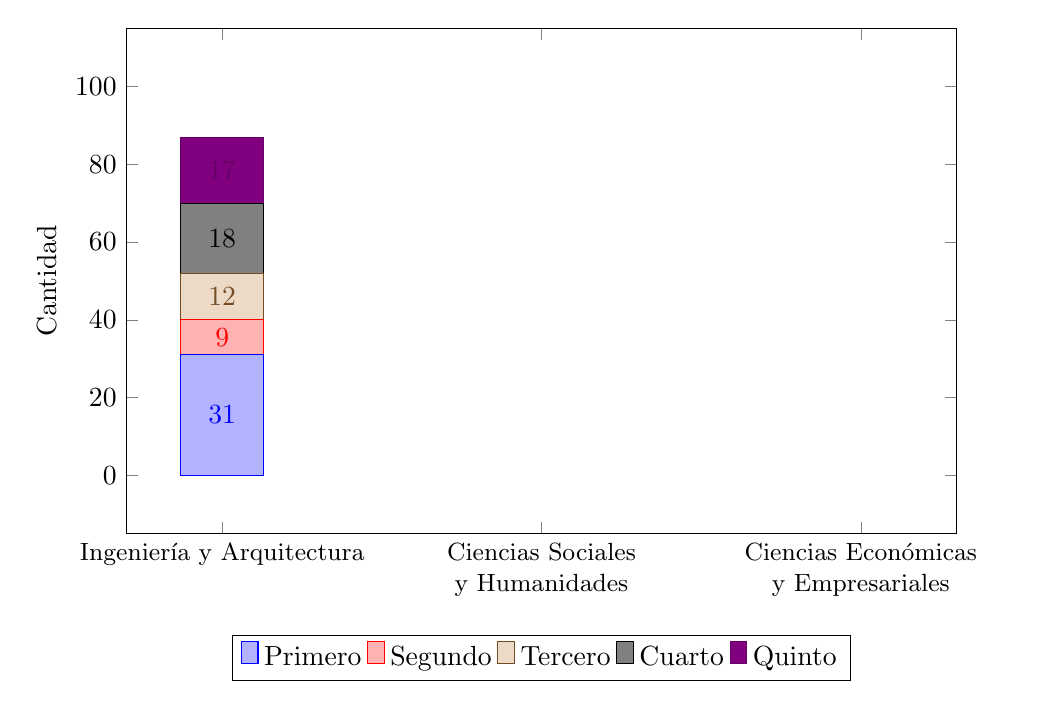
\begin{tikzpicture}
                \begin{axis}[
                    ybar stacked,
                    bar width=30pt,
                    nodes near coords,
                    enlargelimits=0.15,
                    legend style={at={(0.5,-0.2)}, anchor=north, legend columns=-1},
                    ylabel={Cantidad},
                    symbolic x coords={Ingeniería y Arquitectura, Ciencias Sociales y Humanidades, Ciencias Económicas y Empresariales},
                    xtick=data,
                    x tick label style={rotate=0, anchor=north, align=center, text width=4cm, font=\small},
                    ymin=0,
                    ymax=100,
                    width=\textwidth,
                    height=8cm
                ]
                \addplot coordinates {(Ingeniería y Arquitectura,31) (Ciencias Sociales y Humanidades,0) (Ciencias Económicas y Empresariales,0)};
                \addplot coordinates {(Ingeniería y Arquitectura,9) (Ciencias Sociales y Humanidades,0) (Ciencias Económicas y Empresariales,0)};
                \addplot coordinates {(Ingeniería y Arquitectura,12) (Ciencias Sociales y Humanidades,0) (Ciencias Económicas y Empresariales,0)};
                \addplot coordinates {(Ingeniería y Arquitectura,18) (Ciencias Sociales y Humanidades,0) (Ciencias Económicas y Empresariales,0)};
                \addplot coordinates {(Ingeniería y Arquitectura,17) (Ciencias Sociales y Humanidades,0) (Ciencias Económicas y Empresariales,0)};
                \legend{Primero, Segundo, Tercero, Cuarto, Quinto}
                \end{axis}
            \end{tikzpicture}
            \caption{Año de carrera y Facultad del gráfico}
            \label{fig:anio_facultad}
        \end{figure}

        La composición de la muestra se alineo bien con el objetivo del estudio, ya que la mayor parte de los que respondieron la encuesta fueron estudiantes de primer año (35.63\%), todos pertenecientes a la Facultad de Ingeniería y Arquitectura (100\%). Queremos que UCAChat está especialmente orientado a apoyar a estudiantes de nuevo ingreso, quienes enfrentan mayor incertidumbre respecto a procesos institucionales clave como retiro de materias, diferidos, inscripción y ubicación de información académica. Dado que estos estudiantes son quienes más requieren orientación en su transición universitaria, la muestra resultante es coherente y adecuada para los fines de la investigación, garantizando que las conclusiones reflejen las necesidades de los estudiantes que más se beneficiará con la implementación de UCAchat.
    }
    \capitulo{Formato de los trabajos}{
    A continuación, se muestran las características principales del formato de trabajos de graduación creado por la facultad de ingeniería y arquitectura de la UCA.
    
    \begin{lista}
        \item \textbf{Partes del documento:}
        \begin{lista}
            \item Primera portada.
            \item Segunda portada.
            \item Agradecimientos (opcional).
            \item Dedicatorias (opcional).
            \item Resumen.
            \item Índice.
            \item Índice de figuras.
            \item Índice de tablas.
            \item Siglas.
            \item Abreviaturas.
            \item Nomenclatura.
            \item Capítulos.
            \item Glosario (opcional).
            \item Referencias.
            \item Anexos.
        \end{lista}

        \item \textbf{Formato general:}
        \begin{lista}
            \item Pagina tamaño carta.
            \item Margen de 2.5cm en todos lados.
            \item Borde de encuadernación de 1cm.
            \item Fuente Times New Roman 11pt.
            \item Interlineado 1.5pt.
            \item Espacio extra entre párrafos 0.
            \item Línea vacía entre párrafos.
            \item Todas las secciones deben comenzar en página impar.
            \item En todas las secciones que llevan título, el titulo se coloca al inicio de la página, en negrita, en mayúscula y centrado horizontalmente.
            \item Debe haber separación de una línea vacía entre el título y el texto.
        \end{lista}

        \item \textbf{Portadas:}
        \begin{lista}
            \item Texto centrado horizontalmente.
            \item Espacio igual entre los párrafos para que el texto ocupe todo el espacio disponible.
            \item Texto en mayúscula.
            \item Fuente tamaño 14pt.
            \item Logo de la primera portada 2.5cm de alto.
            \item En la primera portada los nombres de los integrantes van ordenados en orden alfabético basados en el primer apellido.
    \end{lista}

    \item \textbf{Agradecimientos:}
    \begin{lista}
        \item Extensión máxima una página.
    \end{lista}

    \item \textbf{Dedicatoria:}
    \begin{lista}
        \item Una por cada integrante.
        \item Extensión máxima una página.
        \item Debe llevar el nombre correspondiente del integrante al final de la página y alineado al lado derecho.
    \end{lista}

    \item \textbf{Resumen:}
    \begin{lista}
        \item Extensión de una a tres páginas.
    \end{lista}

    \item \textbf{Índice:}
    \begin{lista}
        \item El espacio horizontal entre el nombre de las secciones y el número de página debe estar lleno de puntos.
        \item Se permite hasta tres niveles de título.
        \item Los títulos de las secciones principales van en mayúscula.
        \item Al final se deben colocarlos anexos.
    \end{lista}

    \item \textbf{Índice de figuras e índice de tablas:}
    \begin{lista}
        \item Cada entrada del índice de figuras debe iniciar con la palabra “Figura” seguido del número de capitulo y el número correlativo de la figura.
        \item Cada entrada del índice de tablas debe iniciar con la palabra “Tabla” seguido del número de capitulo y el número correlativo de la tabla.
    \end{lista}

    \item\textbf{Siglas, abreviaturas y nomenclatura:}
    \begin{lista}
        \item Van separados en dos columnas, en la columna izquierda se coloca la sigla o palabra seguido de dos puntos y en la columna derecha se coloca la definición.
    \end{lista}

    \item\textbf{Figuras:}
    \begin{lista}
        \item Las figuras incluyen gráficos, diagramas, fotos, etc.
        \item El epígrafe va en la parte inferior centrado horizontalmente.
        \item Al inicio va la palabra “Figura” seguido del número de capitulo y número correlativo.
        \item En el epígrafe continuo a la descripción de la figura va la fuente.
        \item La fuente sigue el siguiente formato, “Fuente: [apellido autor, año]”.
        \item Si la figura es de elaboración propia se coloca, “Fuente: [Elaboración propia]”.
        \item Si la figura ha sido adaptada de alguna parte se coloca, “Adaptado de: [apellido autor, año]”.
        \item Las figuras se pueden colocar con orientación horizontal, en ese caso siempre de izquierda a derecha.
        \item Si la figura tiene orientación horizontal, el epígrafe se coloca en el lado derecho de la página.
    \end{lista}

    \item\textbf{Tabla:}
    \begin{lista}
        \item El epígrafe va en la parte superior, centrado horizontalmente.
        \item Al inicio va la palabra “Tabla” seguido del número de capitulo y número correlativo.
        \item La fuente se coloca en la parte inferior, centrada horizontalmente.
        \item La fuente sigue el siguiente formato, “Fuente: [apellido autor, año]”.
        \item Si la tabla es de elaboración propia se coloca, “Fuente: [Elaboración propia]”.
        \item Si la figura ha sido adaptada de alguna parte se coloca, “Adaptado de: [apellido autor, año]”.
        \item Las tablas se pueden colocar con orientación horizontal, en ese caso siempre de izquierda a derecha.
        \item Si la tabla tiene orientación horizontal, el epígrafe se coloca en el lado izquierdo de la página.
    \end{lista}

    \item\textbf{Ecuaciones:}
    \begin{lista}
        \item Las ecuaciones deben estar numeradas de la siguiente forma “(Ec.1.1)”.
    \end{lista}

    \item \textbf{Glosario:}
    \begin{lista}
        \item Tiene el mismo formato que las siglas, abreviaturas y nomenclatura.
    \end{lista}

    \item\textbf{Referencia:}
    \begin{lista}
        \item El formato de la referencia es en formato APA.
        \item No se coloca sangría en las líneas de cada una de las referencias.
        \item Las referencias van separadas horizontalmente por una línea vacía.
    \end{lista}

    \item\textbf{Portada anexos:}
    \begin{lista}
        \item Los anexos se enumeran utilizando letras.
        \item La portada de los anexos lleva dos partes, lleva la palabra “ANEXO” en mayúscula seguido de la letra correspondiente, el tamaño de fuente de esta parte es 20pt.
        \item El título del anexo en mayúscula, el tamaño de fuente de esta parte es 16pt.
        \item Todo el texto va centrado vertical y horizontalmente.
    \end{lista}

    \end{lista}
    }
}

%=================================================================
%       Sección editable para conclusiones y recomendaciones
% ================================================================
% ================= NO MODIFICAR LOS COMANDOS ===================
% ================================================================

\newenvironment{conclusiones}{En esta sección se escriben las conclusiones a las que se ha llegado luego de realizar el trabajo, las conclusiones deben concordar con los objetivos planteados anteriormente.}{}

\newenvironment{recomendaciones}{
En esta sección, se presentan las recomendaciones hechas por el grupo de trabajo para las personas que se beneficiarán del estudio o proyecto realizado.
}{}

%=================================================================
%                Sección editable para glosario
% ================================================================
% ================= NO MODIFICAR LOS COMANDOS ====================
% ================================================================

\newcommand{\mostrarglosario}{true}
\itemglosario{Glosario}{En esta sección, se incluyen términos utilizados en el documento cuya definición podría\newline no ser conocida por el lector, especialmente aquellos de carácter técnico. Esta sección\newline es opcional, como por ejemplo: BackEnd (Parte de una aplicación web que gestiona\newline la lógica, el procesamiento de datos y la comunicación con el servidor).}
\itemglosario{}{}
\itemglosario{}{}

%=================================================================
%                    Sección editable para anexos
% ===============================================================
% ================== NO MODIFICAR LOS COMANDOS ==================
% ================================================================

\newcommand{\anexos}{
    \anexo{anexos}{
     En los anexos se colocan los documentos, gráficos, tablas, imágenes u otros materiales complementarios que proporcionan información adicional relevante, pero que no forman parte del cuerpo principal del trabajo.
    }
}

